% secdoc.tex V2.0, 28 June 2010

\documentclass[times]{secauth}

\usepackage{moreverb}

\usepackage[colorlinks,bookmarksopen,bookmarksnumbered,citecolor=red,urlcolor=red]{hyperref}

%\usepackage{multirow}
%\usepackage{multicol}

\usepackage{mcite}
\usepackage{graphicx}
\usepackage{float}
\usepackage{leftidx}
\usepackage{amssymb}
\usepackage[caption=false]{subfig}
\usepackage{bm}
\usepackage{array}
\usepackage{enumerate}
\usepackage{url}
\usepackage{amsmath}
\usepackage{amsthm}
\newtheorem{theorem}{Theorem}[section]
\newtheorem{lemma}[theorem]{Lemma}
%
\usepackage{cite}
%
\theoremstyle{definition}
\newtheorem{definition}[theorem]{Definition}
\theoremstyle{remark}
\newtheorem{remark}[theorem]{Remark}

\newcommand{\tabincell}[2]{\begin{tabular}{@{}#1@{}}#2\end{tabular}}

\newcommand\BibTeX{{\rmfamily B\kern-.05em \textsc{i\kern-.025em b}\kern-.08em
T\kern-.1667em\lower.7ex\hbox{E}\kern-.125emX}}

\def\volumeyear{2010}

\begin{document}

\runningheads{P.~Chen.~Other}{An EF-HIBOOS Scheme for Privacy Protection of PCS}

\articletype{RESEARCH ARTICLE}

\title{An Escrow-Free Online/Offline HIBS Scheme for Privacy Protection of People-Centric Sensing}

\author{Peixin Chen$^1$, Jinshu Su$^{2, 1}$, Baokang Zhao$^1$, Xiaofeng Wang$^1$ and Ilsun You$^3$\corrauth}

\address{$^1$ College of Computer, National University of Defense Technology, Changsha 410073, China\\
$^2$ National Key Laboratory for Parallel and Distributed Processing, National University of Defense Technology, Changsha 410073, China\\
$^3$ Department of Information Security Engineering, Soonchunhyang University, Asan-si, Republic of Korea}

\corraddr{Department of Information Security Engineering, Soonchunhyang University, Asan-si, Republic of Korea.}

\begin{abstract}
People-Centric Sensing (PCS), which collects information closely related to human activity and interactions in societies, is stepping into a flourishing time. 
Along with its great benefits, PCS poses new security challenges such as data integrity, participant privacy. 
Hierarchical Identity-Based Signature (HIBS) scheme can efficiently provide high integrity messaging, secure communication and privacy protection to PCS.
However, key escrow problem and low computation efficiency primarily hinder the adoption of HIBS scheme.
In this paper, we propose an escrow-free online/offline HIBS (EF-HIBOOS) scheme for securing PCS.
By utilizing user-selected-secret signing algorithm and splitting the signing phase into online and offline procedures, our scheme solves the key escrow problem and achieve high scheme performance.
\end{abstract}

\keywords{Internet of Things; People-Centric Sensing; Hierarchical Identity-Based Signature; Online/Offline Signature; Key Escrow Problem}

\maketitle

\footnotetext[2]{Please ensure that you use the most up to date
class file, available from the SEC Home Page at\\
{\tiny\href{http://www3.interscience.wiley.com/journal/114299116/home}{\texttt{http://www3.interscience.wiley.com/journal/114299116/home}}}}

\section{Introduction} 
With enormous improvements of sensing technology and embed computation, more and more ubiquitous devices are utilized to build a new kind of mobile sensing system, which is referred to as People-Centric Sensing (PCS) system \cite{campbell2008rise}. 
However, the PCS is facing a more serious privacy problem than the traditional wireless sensor network.
Works on protecting the privacy of PCS has been proposed \cite{cornelius2008anonysense,shi2010prisense,puttaswamy2010preserving,johnson2007people}. 
Most of the work assume that participant of PCS application are supported from a public key infrastructure (PKI).
Nevertheless, building and operating a PKI are quite burden jobs, which significantly reduce the practicability of the PKI-based scheme.
The Identity-Based Signature (IBS) scheme can be efficiently utilized to build a lightweight PKI that is appropriate for the PCS application.
\par 

IBS is a public key signature scheme which allows a receiver to verify message using the signer's identity as the public key \cite{shamir1985identity}. Choon et al. propose the first practical IBS scheme that utilizes a Private Key Generator (PKG) to generate private key for users \cite{choon2002identity}.
On this basis, Gentry et al. present the first Hierarchical IBS (HIBS) scheme, which greatly reduces the workload on PKG and resolves the problem of single-point failure in IBS scheme \cite{gentry2002hierarchical}. 
Improving the scheme security and efficiency, several IBS and hierarchical IBS (HIBS) schemes \cite{boneh2001short,boneh2004short,chow2004secure,camenisch2004signature,yao2014novel,gerbush2012dual} have been presented. 
\par

Deployment of an HIBS scheme has to take two problems into consideration: key escrow problem and scheme performance problem. 
Since an HIBS scheme uses PKGs to generate private key for users, it inevitably leads to the \emph{key escrow problem}. 
That is, the PKG knows the private keys and thus can unscrupulously sign messages intended for the users \cite{boneh2001identity}. 
Besides the key escrow problem, the low computation efficiency of HIBS scheme is another concern while deploying the identity-based signature scheme.
Most IBS schemes involve computations including pairings over points on elliptic cure and point multiplications in groups, which might be too costly to be applied in lightweight devices.
Online/offline (OO) signature mechanism that divides the process of message signing into offline phase and online phase is an effective method to reduce the computational cost of signature generation \cite{even1990line}. 
The offline phase is performed prior to the knowledge of the message to be signed, and the online phase is performed after knowing the message. 
In an OO mechanism, most of the computation is implemented in offline signing and online signing is typically very fast while generating a signature.
Imposing the OO mechanism, numerous identity-based online/offline signature (IBOOS) scheme have been proposed \cite{yang2013id,liu2011online,yasmin2010authentication,liu2010efficient,kar2014provably,lai2015improved}. 
Yang et al. present a comprehensive IBOOS scheme, which solves the key escrow problem utilizing a threshold model and achieves high performance thanks to the OO signing algorithm \cite{yang2013id}.
However, there are few work on hierarchical IBOOS (HIBOOS) scheme and its key escrow problem.  
\par

In this paper, we propose an escrow-free online/offline hierarchical identity-based signature (EF-HIBOOS) scheme, which only executes two group element exponentiation operations in online procedure. 
We use a user-selected secret besides the signing key to sign messages so that any bogus signatures can be recognized and forgery behaviors can be detected and blamed. 
We prove that our scheme is selective-identity and adaptive chosen-message secure for existential-forgery attack (EF-sID-CMA) secure and can efficiently solve the key escrow problem.
\par

The rest of this paper is organized as follows.
We overview our escrow-free HIBOOS model in Section \ref{sec-overview}. 
The construction and security proof of the HIBOOS scheme are presented in Section \ref{sec-EFOOHIBS}. 
We discuss the performance and advantages of our HIBOOS scheme in Section \ref{sec-Performance}.
Related works are reviewed in Section \ref{sec-relatedwork} and our work is concluded in Section \ref{sec-conclusion}.

\section{Overview of our escrow free HIBOOS model}\label{sec-overview}
In this section, we firstly review some background knowledge, including the bilinear pairing and the complexity assumption used in our proof.
Then, we introduce the intuition of our solution to the key escrow problem of HIBOOS, and briefly describe the construction of our scheme. 
Finally, we present the security definition by illuminating the \emph{EF-sID-CMA}, \emph{EKA-ID-CMA} and \emph{EUS-sID-CMA} attack games for our escrow-free approach.

\subsection{Preliminaries}\label{sec-Pre}
\subsubsection{Bilinear Pairing}\label{sec-bilinearpairing}
Let $G_1$ and $G_2$ be two cyclic multiplicative groups of the same order $p$. 
A map $e: G_1 \times G_1 \rightarrow G_2$ is referred to as a bilinear paring if it has the following properties: 
\begin{enumerate}[1.]
\item Bilinear: $\forall u,v \in G_1, a,b \in \mathbb{Z}_N$, there is $e(u^a, v^b) = e(u,v)^{ab} $;
\item Non-degenerate: $\exists g \in G_1$, s.t. $e(g,g) \neq 1$, where $1$ denotes the identity in $G_2$;
\item Computable: $\forall u, v \in G_1$, there is an efficient algorithm to compute $e(u,v)$.
\end{enumerate}

\subsubsection{Complexity Assumption}
We prove the security of our scheme based on the CDH assumption. 
The assumption is defined as follows: 
\begin{definition}[CDH Assumption]
Let $G$ be a cyclic multiplicative group generated by $g$ and $a, b \in \mathbb{Z}_p$.
Given $g, g^a, g^b$, there is no probabilistic polynomial time algorithm $\mathcal{A}$ has a non-negligible advantage to compute the value $g^{ab}$.
\end{definition}

\subsection{Intuition of Escrow-free}
In the HIBOOS scheme, a user private key is generated by a domain PKG. 
Therefore, either the domain PKG or the user can sign a message to obtain a valid signature. 
Since the signature verifier cannot determine the actual signer, two problems should be addressed in those primitive HIBS scheme:
\begin{itemize}
\item \emph{Key abusing problem}. A domain PKG is able to sign messages with the user keys generated by it without being detected;
\item \emph{User slandering problem}. The dishonest user is able to sign a message and slander that the PKG abuses its private key. That is, the undeniable property is missing in the primitive HIBS scheme. 
\end{itemize}
\par 
For the key abusing problem, an intuitive solution is to limit the signing ability of the PKG by a well designed signing algorithm.
Therefore, we use a user-selected secret apart from the private key to generate the signature for a message. 
We also compute a user public parameter with the secret as input.
The user sends the parameter along with the message and signature to the receivers. 
Signature verifying needs to take user parameter and signature as input. 
Since the PKG cannot obtain the user secret, it cannot generate a valid signature with respect to the user parameter. 
However, the PKG can generate a well-formed signature with a fake user parameter. 
Receiver will thereby accept the PKG generated signature-parameter pair. 
To solve such problem, we introduce an Arbitral Party (AP) to keep the users' public parameters.
User publishes its user parameter, and attaches these same parameter to each signature.
A receiver is not constrained to compare the user parameter attaching in the signature with the one publishing in the AP.
Nevertheless, the PKG will be detected and blamed once it abuses a user private key to sign messages. 
Note that, an AP does not keep any confidential contents.
\par
Since PKG is able to generate well-formed signatures with distinct user parameters, a user can slander the PKG by signing messages with randomly picked secret and sending the receiver a corresponding fake user parameter along with the signature. 
To solve this problem, we modify the signing algorithm so that the user can only generate well-formed signatures with regard to the parameter it published. 
After publishing the public parameter, user also needs to ask for a PKG signing factor from the root PKG. 
The root PKG computes the factor with the user parameter as well as the master secret as input and returns the factor to the user.
User is desired to sign messages with the PKG signing factor. 
\par 
Combining these two technologies, we can present a full secure escrow-free HIBS model. 
Generally speaking, it can be applied to any secure HIBS schemes by modifying the signing and verifying algorithms.
In this paper, we instantiate an escrow-free HIBOOS scheme with the above intuition. 
The construction and security proof are described in Section \ref{sec-EFOOHIBS}.

\subsection{Generic Construction}
\begin{figure*}
\centering
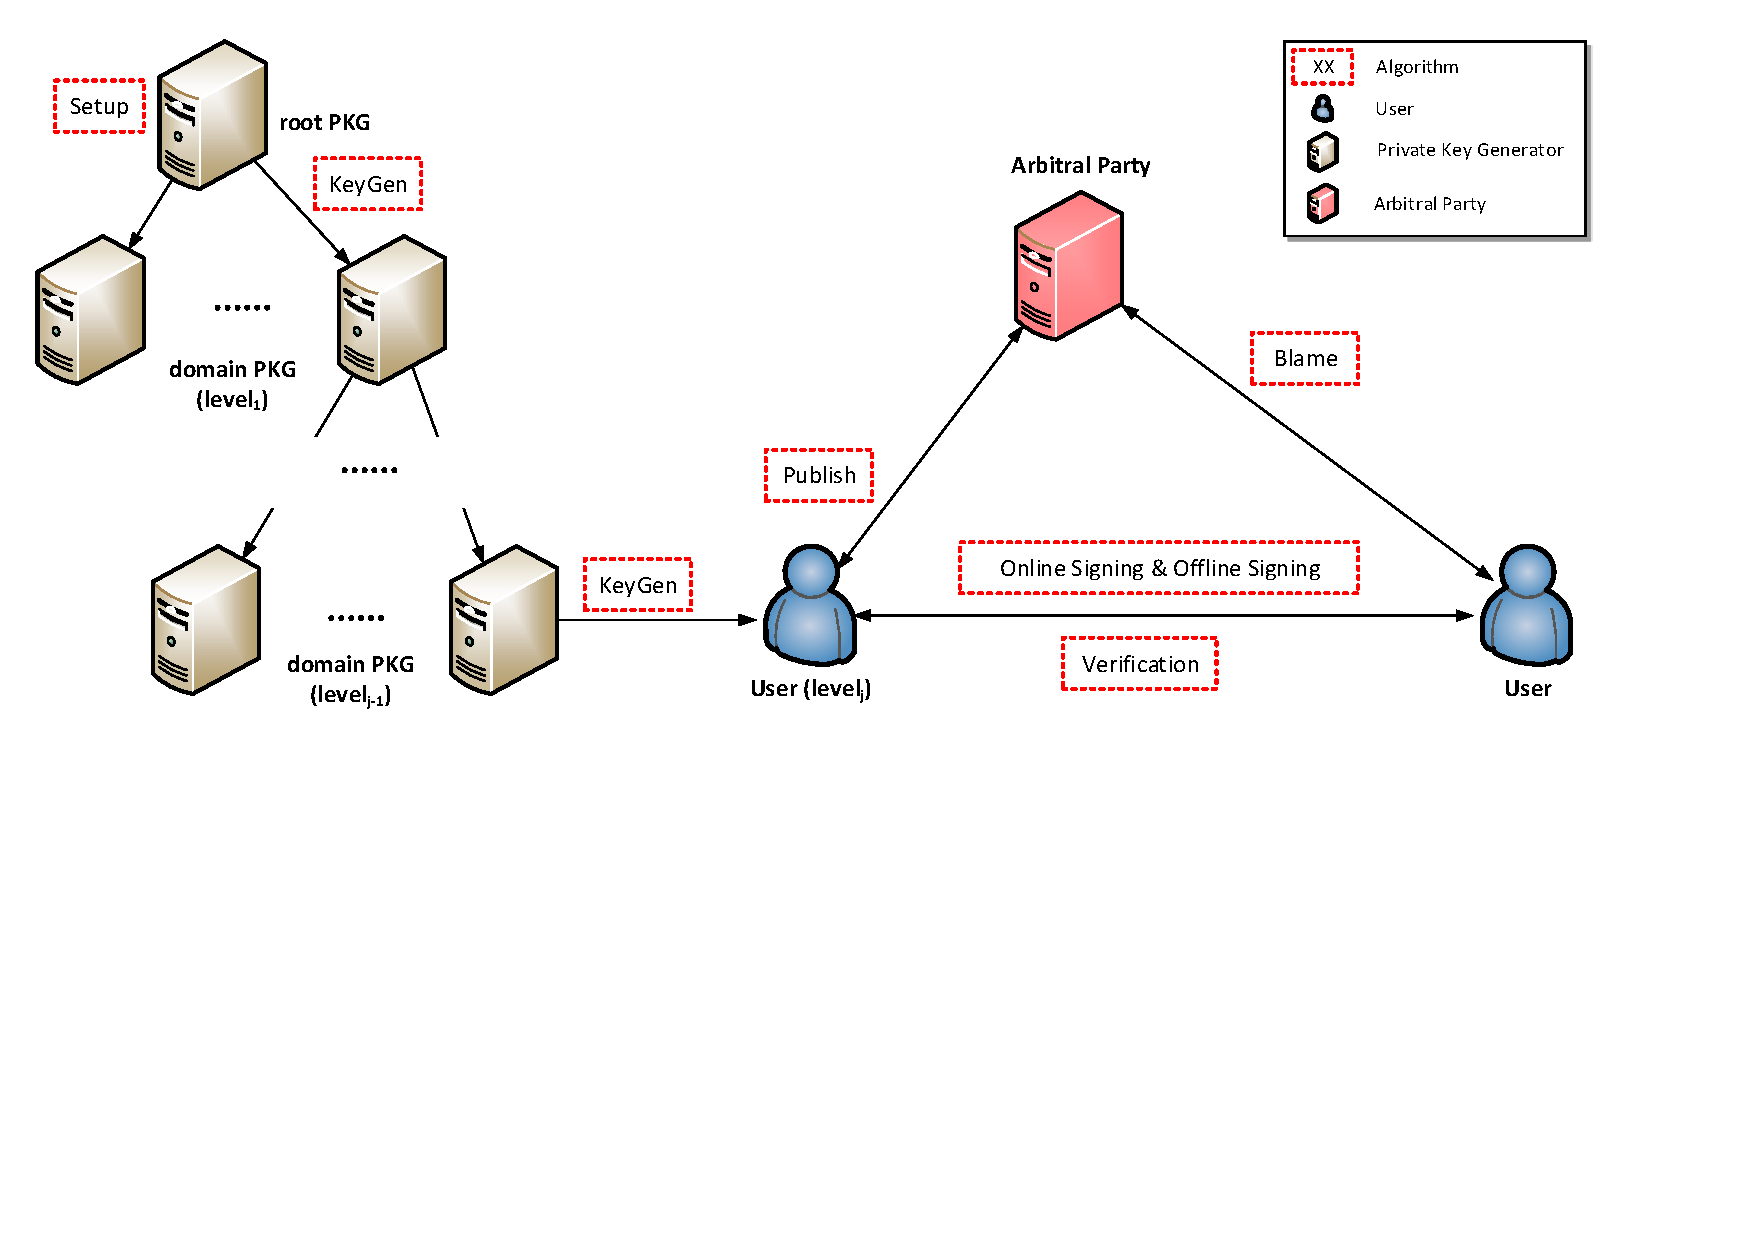
\includegraphics[width=15cm]{schema.pdf}
\caption{Generic construction of the HIBOOS scheme.} \label{fig-schema}
\end{figure*}
A primitive hierarchical identity-based online/offline signature scheme generally consists of five algorithms: Setup, KeyGen, Offline Signing, Offline Signing and Verification.
To achieve the escrow-free property, we add Publish algorithm and Blame algorithm to our HIBOOS scheme.
The generic construction of our HIBOOS scheme is shown as in Figure \ref{fig-schema}. 
The scheme consists of the following 7 algorithms:
\vspace{0.1cm}
\\
\textbf{Setup.}
The setup algorithm takes a security parameter as input and outputs the HIBS public parameters. 
\vspace{0.1cm}
\\
\textbf{KeyGen.}
The key generation algorithm takes a secret key and an identity ID as input and outputs the user private key. 
More specifically, the root PKG takes the master secret as input and can generate private keys for any user.
Each domain PKG takes its private key as input and generates private keys for its descendant user.
\vspace{0.1cm}
\\
\textbf{Publish.}
The algorithm takes the user secret as input and outputs the user parameter. 
User uploads the parameter to the AP and get PKG signing factor from the root PKG.
\vspace{0.1cm}
\\
\textbf{Offline Signing.}
The offline signing algorithm is performed prior to obtaining the message. 
It takes a private key as well as the public parameter as input, and outputs the offline signature.
\\
\textbf{Online Signing.}
The online signing algorithm takes a message, a private key and the offline signature as input, and outputs a final signature.
\vspace{0.1cm}
\\
\textbf{Verification.}
The verification algorithm takes an identity $\mathrm{ID}$, a message $m$ and a signature as input.
If $\sigma$ is valid, outputs 1. 
Otherwise, outputs 0.
\vspace{0.1cm}
\\
\textbf{Blame.}. 
The algorithm takes a message-signature pair $\{m, \sigma\}$  and a user parameter as input.
If $\sigma$ is generated by an honest signer, outputs 0.
Otherwise, outputs 1.

\subsection{Security Model}
We claim that an secure escrow-free hierarchical identity-based online/offline signature scheme should be uncrackable against three attack games: \emph{EF-sID-CMA}, \emph{EKA-ID-CMA} and \emph{EUS-sID-CMA}. 
\par

\begin{definition}[\emph{EF-sID-CMA} Security]
We say that a hierarchical identity-based online/offline signature scheme is secure if no probabilistic polynomial time (\emph{PPT}) adversary $\mathcal{A}$ has a non-negligible advantage against the challenger $\mathcal{C}$ in the above \emph{EF-sID-CMA} game. 
As shorthand, we say that the HIBS scheme is \emph{EF-sID-CMA} secure.
\end{definition}
\par
\begin{definition}[\emph{EKA-ID-CMA} Security]
We say that a hierarchical identity-based online/offline signature scheme is secure if no \emph{PPT} adversary $\mathcal{A}$ has a non-negligible advantage against the challenger $\mathcal{C}$ in the above \emph{EKA-ID-CMA} game. 
As shorthand, we say that the HIBS scheme is \emph{EKA-ID-CMA} secure.
\end{definition}
\begin{definition}[\emph{EUS-sID-CMA} Security]
We say that a hierarchical identity-based online/offline signature scheme is secure if no \emph{PPT} adversary $\mathcal{A}$ has a non-negligible advantage against the challenger $\mathcal{C}$ in the above \emph{EUS-ID-CMA} game. 
As shorthand, we say that the HIBS scheme is \emph{EUS-sID-CMA} secure.
\end{definition}
\par
Details of the security model can be found in our previous work \cite{anescrowfree2015chen}.
%We highlight some important notes of the games as follows:
%\begin{itemize}
%	\item 
%	\item 
%\end{itemize}

\section{Escrow-free Online/Offline HIBS Scheme}\label{sec-EFOOHIBS}
In this section, we present the construction of our escrow-free HIBOOS scheme, and prove the security of our scheme via there attack games.

\subsection{Construction}
Let $K$ be the security parameter given to the setup algorithm, and let $\mathcal{G}$ be a BDH parameter generator.
 %\vspace{0.2cm}
\\
\textbf{Setup.} Given a security parameter, the PKG works as follows:
\begin{enumerate}
\item runs $\mathcal{G}$ on input $K$ to generate multiplicative groups $G_1, G_2$ of same prime order, and a bilinear pairing $\hat{e}: G_1 \times G_1 \rightarrow G_2$;
\item chooses random $\alpha \in \mathbb{Z}^*_p$ and two generators $g, g_2 \in G_1$, computes $g_1 = g^\alpha$;
\item randomly picks $h_1, \ldots, h_\ell \in G_1$;
\item chooses two cryptographic hash functions $H_1: \{0, 1\}^* \times G_1 \rightarrow \mathbb{Z}_p^*$ and $H_2: G_1 \times \{0, 1\}^* \rightarrow G_1$;
\item publishes $Param = \{\hat{e}, g, g_1,  g_2, h_1, \ldots, h_\ell, H_1, \\H_2\}$ as public parameters and keeps $\mathrm{MSK} = g_2^\alpha$ as master secret.
\end{enumerate}
\textbf{KeyGen.} For an input $\mathrm{ID} = \{I_1, \ldots, I_k\}$, the $level_{k-1}$ domain PKG with private key $d_{\mathrm{ID}_{\mid k-1}} = \{d'_0, \ldots, d'_{k-1}\}$ generates the key $d_\mathrm{ID}$ as follows:
\begin{enumerate}
\item picks random $r_k \in \mathbb{Z}_p^*$;
\item set $d_{\mathrm{ID}} = \{d'_0F_k(I_k)^{r_k}, d'_1, \ldots, d'_{k-1}, g^{r_k}\}$,\\ where $F_k(x)$ $ = g_1^xh_k$.
\end{enumerate}
\par
We refer to $g_2^\alpha$ as $d_{\mathrm{ID}_{\mid 0}}$, and the user private key can be presented as 
$d_{\mathrm{ID}} = \{d_0, d_1, \ldots, d_k\} = \{g_2^\alpha \prod^k_{j=1} F_j(I_j)^{r_j},$ $g^{r_1}, \ldots, g^{r_k}\}$.
\vspace{0.2cm}
\\
\textbf{Publish.} In this phase, user publishes a public parameter and gets PKG signing factor from the root PKG. 
It does the work as follows:
\begin{enumerate}
\item randomly picks $s_{\mathrm{ID}} \in \mathbb{Z}_p^*$ as user secret;
\item computes $g_{\mathrm{ID}} = g^{s_{\mathrm{ID}}}$;
\item publishes $g_{\mathrm{ID}}$ by submitting it to the AP;
\item sends $g_{\mathrm{ID}}$ to the root PKG, the root PKG computes and returns $f^\alpha = H_2(g_\mathrm{ID}, \mathrm{ID})^\alpha$. 
\end{enumerate}
Although the root PKG has to computes the signing factor for all users, it brings in little overhead because of the following reasons:
\begin{itemize}
\item it has not to authenticate the users before computing the signing factors for them;
\item it has not to maintain a secure channel to transmit the signing factor;
\item it only needs to do an exponentiation computation for each user.
\end{itemize}
\textbf{Offline Signing.} 
During this phase, the signer computes the followings:
To sign a message $m \in \{0, 1\}^*$ with respect to identity $\mathrm{ID} = \{I_1, \ldots, I_k\}$, user takes the private key $d_{\mathrm{ID}} = \{d_0, d_1, \ldots, d_k\}$, secret $s_{\mathrm{ID}}$ and PKG signing factor $f^\alpha$ as input, running the signing algorithm as follows:
\begin{enumerate}
\item picks a random $s \in \mathbb{Z}_p^*$ and computes $x = g_2^s$;
\item for $j = 1, \ldots, k$, computes $y_j = d_j^{s}$;
%\item computes $d_0^{s}$;
\item computes $f = H_2(g_\mathrm{ID}, \mathrm{ID})$;
\item computes\\$E_{off} = \hat{e}(g_1, \prod_{j=1}^{k} d_j^{I_j})\prod_{j=1}^{k} \hat{e}(d_j, h_j)$;
\item computes $z_{off} = d_0^sf^{s_\mathrm{ID}} f^\alpha = d_0^sf^{s_\mathrm{ID} + \alpha}$;
\item sets the offline signature as $\sigma_{off} = \{x, y_1, \ldots, y_k, \\z_{off}, E_{off}, g_{\mathrm{ID}}\}$.
\end{enumerate}
\textbf{Online Signing.}
During this phase, the signer computes the followings:
\begin{enumerate}
\item computes  $h = H_1(m, x)$;
\item computes $z = d_0^h z_{off} =  d_0^{s+h}f^{(s_\mathrm{ID} + \alpha)}$;
\item computes $E=E_{off}^h$;
\item sets signature as $\sigma_{on} = \{z, E\}$.
\end{enumerate}
\par
The signature is $\sigma = \{x, y_1, \ldots, y_k, z, E, g_{\mathrm{ID}}\}$.
\vspace{0.2cm}
\\
\textbf{Verification.} To verify $\sigma = \{x, y_1, \ldots, y_k, z, E, g_{\mathrm{ID}}\}$ on message $m$ with respect to identity $\mathrm{ID} = \{I_1, \ldots, I_k\}$, the verification algorithm works as follows:
\begin{enumerate}
\item computes $h = H_1(m, x)$ and $f = H_2(g_\mathrm{ID}, \mathrm{ID})$;
\item checks whether the equation holds:
$\hat{e}(g, z) = E \cdot \\ \hat{e}(g_1, g_2^hx\prod_{j=1}^k y_j^{I_j})\hat{e}(f, g_\mathrm{ID}g_1)\prod_{j=1}^k \hat{e}(y_j, h_j)$\\
If so, outputs 1. Otherwise, outputs 0.
\end{enumerate}
\par
Actually, if the signature is valid, there is 
\begin{align*}
&E \cdot \hat{e}(g_1, g_2^hx\prod_{j=1}^k y_j^{I_j})\hat{e}(f, g_\mathrm{ID}g_1)\prod_{j=1}^k \hat{e}(y_j, h_j)\\
=&\hat{e}(g_1, \prod_{j=1}^{k} d_j^{I_j})^h \left(\prod_{j=1}^{k} \hat{e}(d_j, h_j)^h\right)\hat{e}(g_1, g_2^{(s+h)}\prod_{j=1}^k y_j^{I_j}) \cdot\\
&\hat{e}(f, g_\mathrm{ID}g_1)\prod_{j=1}^k \hat{e}(y_j, h_j)\\
=&\hat{e}(g_1, g_2^{(s+h)}\prod_{j=1}^k d_j^{(s+h)I_j}) \hat{e}(f, g^{s_\mathrm{ID}}g^\alpha) \prod_{j=1}^{k} \hat{e}(d_j^{(s+h)}, h_j)\\
=&\left(\hat{e}(g^\alpha, g_2g^{\sum_{j=1}^kr_jI_j})\hat{e}(\prod_{j=1}^{k} g, h_j^{r_j})\right)^{(s+h)}\hat{e}(g, f^{s_\mathrm{ID}}f^\alpha)\\
=&\hat{e}(g,g_2^\alpha \prod_{j=1}^{k}g_1^{r_jI_j}h_j^{r_j})^{(s+h)}\hat{e}(g, f^{(s_\mathrm{ID}+\alpha)})\\
=&\hat{e}(g,d_0^{(s+h)}f^{(s_\mathrm{ID}+\alpha)})\\
=&\hat{e}(g, z).
\end{align*}
Note that, although the user public parameter is carried as a part of the signature, the receiver is not constrained to verify whether the signature is generated by the user by checking the parameter. 
That is, the receiver implicitly believes a message is signed by the sender if the signature is correctly verified. 
The sender himself has to run the \emph{Blame} procedure if he argue that the signature  with respect to his identity is bogus. 
\vspace{0.2cm}
\\
\textbf{Blame.} 
Given $\{\mathrm{ID}, m, \sigma = \{x, y_1, \ldots, y_k, z, g_{\mathrm{ID}}\}\}$, the algorithm requires the user parameter $g'_{\mathrm{ID}}$ with respect to the identity ID from the AP. 
It outputs 1 if and only if $g_{\mathrm{ID}} \neq g'_{\mathrm{ID}}$ and 0 otherwise.

\subsection{Security Proof}
The security of our escrow-free HIBOOS scheme is proved according to the following Lemmas. 
\begin{lemma} \label{lemma-ef-hiboos}
If there exists an EF-sID-CMA algorithm $\mathcal{A}$ that has non-negligible advantage against our HIBOOS scheme, 
then there exists an algorithm $\mathcal{B}$ that breaks the CDH assumption with non-negligible advantage.
\end{lemma}
\begin{proof}
We show how to construct algorithm $\mathcal{B}$ to win the \emph{EF-sID-CMA} game against the CDH assumption. 
Given $g, g^a, g^b$, $\mathcal{B}$ interacts with $\mathcal{A}$ as follows:
\vspace{0.1cm}
\\
\textbf{Init.} 
$\mathcal{A}$ selects an identity $\mathrm{ID}^* = \{I^*_1, \ldots, I^*_k\} (k \leqslant \ell)$ which will be used in the challenge phase.  
\vspace{0.1cm}
\\
\textbf{Setup.} 
$\mathcal{B}$ generates a bilinear map $\hat{e}: G_1 \times G_1 \rightarrow G_2$ with $g$ as a generator of $G_1$.
It randomly picks $\alpha_1, \ldots, \alpha_\ell \in \mathbb{Z}^*_p$, and sets $g_1 = g^a$, $g_2 = g^b$, $h_j =g^{-I^*_j\alpha_j}$ for $j = 1, \ldots, \ell$.
Function $F_j : \mathbb{Z}_p \rightarrow G_1$ is defined as $F_j(x)=g_1^xh_j =g_1^{x-I^*_j}g^{\alpha_j}$.
$\mathcal{B}$ also maintains hash oracle $H_1: \{0, 1\}^* \times G_1 \rightarrow \mathbb{Z}_p^*$.
Parameters $\{\hat{e}, g, g_1,  g_2, h_1, \ldots, h_\ell, H_1\}$ are sent to $\mathcal{A}$.
\vspace{0.1cm}
\\
\textbf{Query.} $\mathcal{B}$ answers queries made by $\mathcal{A}$, where $\mathcal{A}$ is allowed to make up to $q_1$ hash queries, $q_2$ key queries and $q_3$ signing queries.
\begin{itemize}
	\item \emph{Hash queries}. 
	$\mathcal{B}$ maintains lists $L_1$ and $L_2$ to store the answers of the $H_1$ and $H_2$ oracle, respectively.
	\begin{itemize}
	\item $\mathcal{A}$ submits the $H_1$ hash query with input $(m, x)$, $\mathcal{B}$ checks the list $L$. 
	If an entry is found, the same answer is returned to $\mathcal{A}$; otherwise, $\mathcal{B}$ randomly picks $h \in \mathbb{Z}_p^*$ and returns it to $\mathcal{A}$.
	$\mathcal{B}$ stores $(m, x, h)$ to the list $L_1$.
	\item $\mathcal{A}$ submits the $H_2$ hash query with input $(g_\mathrm{ID}, \mathrm{ID})$, $\mathcal{B}$ checks the list $L_2$. 
		If an entry for the query is found, the same answer will be returned to $\mathcal{A}$. 
		Otherwise, if $\mathrm{ID} \neq \mathrm{ID}^*$, $\mathcal{B}$ randomly picks $\beta_i \in \mathbb{Z}_p^*$ and sets $f = H_2(g_\mathrm{ID}, \mathrm{ID}) = g^{\beta_i}$; if $\mathrm{ID} = \mathrm{ID}^*$, sets $f = g^b$.
		$\mathcal{B}$ stores $(g_\mathrm{ID}, \mathrm{ID}, \beta_i)$ to the list $L_2$.
	\end{itemize}
	\item \emph{Key queries}. 
	$\mathcal{A}$ submits a private key query with input $\mathrm{ID} = \{I_1, \ldots, I_u\} (u \leqslant \ell)$, where $\mathrm{ID} \neq \mathrm{ID}^*$.
	Let $j$ be the smallest index such that $I_j \neq I^*_j (1 \leqslant j \leqslant u)$, $\mathcal{B}$ randomly picks $r_1, \ldots, r_j \in \mathbb{Z}_p^*$ and sets
	\begin{align*}
	&d_0 = g_2^{\frac{-\alpha_j}{I_j-I^*_j}}\prod_{v=1}^{j}F_v(I_v)^{r_v}, ~d_1=g^{r_1}, ~\ldots, \\
	&d_{j-1}=g^{r_{j-1}}, ~d_j=g_2^{\frac{-1}{I_j-I^*_j}}g^{r_j}.
	\end{align*}
	Note that, there is
	\begin{align*}
	d_j = g_2^{\frac{-1}{I_j-I^*_j}}g^{r_j} = &g^{\frac{-b}{I_j-I^*_j}}g^{r_j} = g^{r_j-\frac{b}{I_j-I^*_j}},\\
	g_2^{\frac{-\alpha_j}{I_j-I^*_j}}F_j(I_j)^{r_j} = &g_2^{\frac{-\alpha_j}{I_j-I^*_j}}(g_1^{I_j-I^*_j}g^{\alpha_j})^{r_j}\\ 
	= &g_2^\alpha(g_1^{I_j-I^*_j}g^{\alpha_j})^{r_k-\frac{b}{I_j-I^*j}} \\
	= &g_2^\alpha F_j(I_j)^{r_j-\frac{b}{I_j-I^*_j}}.
	\end{align*}
	Thus we can get the private key of $\{I_1, \ldots, I_j\}$:
	\begin{align*}
	&d_0 = g_2^\alpha \left(\prod_{v=1}^{j-1}F_v(I_v)^{r_v}\right)F_j(I_j)^{r_j-\frac{b}{I_j-I^*_j}},\\ 
	&d_1=g^{r_1}, \ldots, d_{j-1}=g^{r_{j-1}}, ~d_j=g^{r_j-\frac{b}{I_j-I^*_j}},
	\end{align*}
	Therefore, the private key returned to $\mathcal{A}$ is well-formed.\\
	For each identity whose prefix equals $\{I_1, \ldots, I_j\}$, $\mathcal{B}$ can generate a private key with the key $d_{\mathrm{ID}\mid j}$.
	\item \emph{Signing queries}. 
	$\mathcal{A}$ submits a signing query with $\mathrm{ID} = \{I_1, \ldots, I_k\}$, $g_\mathrm{ID}$ and $m$ as input, where $\mathrm{ID} \neq \mathrm{ID}^*$.
	If $\mathcal{B}$ does not have a private key $d_{\mathrm{ID}}$ with respect to ID, it generates the private key by implementing the \emph{KeyGen} algorithm.	
	$\mathcal{B}$ signs the message $m$ according to the \emph{Offline} and \emph{Online} algorithm, and returns $\mathcal{A}$ the signature.
\end{itemize}
\textbf{Challenge.} 
$\mathcal{A}$ finally outputs $(\mathrm{ID}^*, m^*, \sigma)$, where $ \sigma=\{x, y_1, \ldots, y_k, z, E, g_{\mathrm{ID}}^*\}$. 
Since $\mathcal{A}$ can break our HIBOOS scheme against the \emph{EF-sID-CMA} game, there is $\hat{e}(g, z) = E \cdot \hat{e}(g_1, g_2^hx\prod_{j=1}^k y^{I^*_j}_j)\hat{e}(f, g_\mathrm{ID}^*g_1)\cdot \\ ~~~~~~~~~~~~~~~~~~\prod_{j=1}^k \hat{e}(y_j, h_j)$.
\\
According to the principle of forking lemma \cite{Pointcheval1996security}, $\mathcal{B}$ can replay $\mathcal{A}$ with the same random tape but different choices of $H_1$.
It then obtains two valid signatures $(x, y_1, \ldots, y_k, z, E, g_\mathrm{ID}^*)$ and $(x, y_1, \ldots, y_k, \bar{z}, E, g_\mathrm{ID}^*)$ on message $m^*$ with respect to hash functions $H_1$ and $\bar{H_1}$ having different values $h \neq \bar{h}$ on $(m^*, x)$, respectively. \par
Thus, there is 
\begin{align*}
&\frac{\hat{e}(g, z)}{\hat{e}(g, \bar{z})} = \frac{\hat{e}(g_1, g_2^hx\prod_{j=1}^k y_j^{I_j})}{\hat{e}(g_1, g_2^{\bar{h}}x\prod_{j=1}^k y_j^{I_j})}\\
\Rightarrow~~ &\hat{e}(g, z\bar{z}^{-1}) = \hat{e}(g_1, g_2^{h-\bar{h}})=\hat{e}(g^a, g^{b(h-\bar{h})})\\
\Rightarrow~~ &z\bar{z}^{-1} = g^{ab(h-\bar{h})}\\
\Rightarrow~~ &g^{ab} = (z^*\bar{z}^{-1})^{1/(h-\bar{h})}.
\end{align*}
\par
Therefore, $\mathcal{B}$ can breaks the CDH assumption.
However, Joux and Nguyen have pointed out that the CDH problem in cyclic group is hard \cite{joux2003separating}. 
That is, our HIBOOS scheme is ES-sID-CMA secure.
\end{proof}

\begin{lemma} \label{lemma-eps-hiboos}
If there exists an EKA-ID-CMA algorithm $\mathcal{A}$ that has non-negligible advantage against our HIBOOS scheme, 
then there is an EKA-ID-CMA algorithm $\mathcal{B}$ that breaks the CWS-HIBS scheme with the same advantage.
\end{lemma}
\begin{proof}
Supposing \emph{EKA-sID-CMA} algorithm $\mathcal{A}$ can break our HIBOOS scheme, we show how to construct a PPT algorithm $\mathcal{B}$ to win the EF-sID-CMA game against the CWS-HIBS scheme.
$\mathcal{B}$ is given parameters of CWS-HIBS scheme $parm = \{g, g_1,  g_2, h_1, \ldots, h_\ell, H_1, H_2\}$, where $\hat{e}: G_1 \times G_1 \rightarrow G_2$ is a bilinear map, $g, g_2$ are generators of cyclic multiplicative group $G_1$, and $H_1$ is a hash function. 
As a simulator, $\mathcal{B}$ provides an \emph{EF-sID-CMA} game to $\mathcal{A}$ and uses the final challenge information to break the CWS-HIBS scheme.\\
$\mathcal{A}$ play the game as below:
\vspace{0.2cm}
\\
\textbf{Setup.} 
$\mathcal{B}$ obtains the public parameters $param = \{g, g_1,  g_2, h_1, \ldots, h_\ell, H_1, H_2\}$ of the CWS-HIBS scheme,
Parameters $param$ are sent to $\mathcal{A}$ as the parameters of our HIBOOS scheme.
\vspace{0.2cm}
\\
\textbf{Query.} $\mathcal{B}$ answers queries made by $\mathcal{A}$. 
\begin{itemize}
	\item Key queries. 
	$\mathcal{A}$ submits an identity $\mathrm{ID}$. 
	$\mathcal{B}$ maintains an ID-key list $L$. 
	If the queried key $d_\mathrm{ID}$ is in the list, $\mathcal{B}$ returns $d_{\mathrm{ID}}$ to $\mathcal{A}$.
	Otherwise, $\mathcal{B}$ takes $\mathrm{ID}$ as the input and queries $d_{\mathrm{ID}}$ from the CWS-HIBS scheme, and returns $d_{\mathrm{ID}}$ to $\mathcal{A}$. 
	\item Signing queries. 
	$\mathcal{A}$ submits $\{\mathrm{ID}, m\}$. 
	If $\mathcal{B}$ does not have a private key $d_{\mathrm{ID}}$ with respect to ID, it queries the private key from the CWS-HIBS scheme and picks a random $s_\mathrm{ID} \in \mathbb{Z}_p^*$. 
	$\mathcal{B}$ inputs $d_\mathrm{ID}$ and $s_\mathrm{ID}$ to sign message $m$ using the signing algorithm provided by our HIBOOS scheme, and gets signature $\sigma = \{x, y_1, \ldots, y_k, z, E\}$.
	Signature $\sigma$ are sent to $\mathcal{A}$.
\end{itemize}
\textbf{Challenge.} 
$\mathcal{A}$ finally outputs $(\mathrm{ID}^*, m^*, \sigma)$, where $ \sigma=\{x, y_1, \ldots, y_k, z, E, g_{\mathrm{ID}}^*\}$. 
According to the attack game, there exists a signature query of which the return values is $(\mathrm{ID^*}, m, \sigma)$ with same user public parameter, i.e. $g_{\mathrm{ID}}^* = g_{\mathrm{ID}}$. 
$\mathcal{B}$ retrieves the private key $d_{\mathrm{ID}^*}=\{d_0, \ldots, d_k\}$ of $\mathrm{ID}^*$ from the list $L$.
Since $\mathcal{A}$ can break our HIBOOS scheme against the \emph{EKA-sID-CMA} game, 
there is $\hat{e}(g, z) = E \cdot \hat{e}(g_1, g_2^hx\prod_{j=1}^k y^{I^*_j}_j)\hat{e}(f, g_\mathrm{ID}^*g_1)\prod_{j=1}^k \hat{e}(y_j, h_j)$.
\par
$\mathcal{B}$ computes $h = H_1(m, x)$, and let $y'_j=y_jd_j^h$, for $j=1, \ldots, k$, $x'=x, z' = z$, there is 
\begin{align*}
&\hat{e}(g, z') =\hat{e}(g, z)\\
=&~E \cdot \hat{e}(g_1, g_2^hx\prod_{j=1}^k y^{I^*_j}_j)\hat{e}(f, g_\mathrm{ID}^*g_1)\prod_{j=1}^k \hat{e}(y_j, h_j)\\
=&~\hat{e}(g_1, \prod_{j=1}^{k} d_j^{hI^*_j})\prod_{j=1}^{k} \hat{e}(d_j^h, h_j)\hat{e}(g_1, g_2^hx\prod_{j=1}^k y^{I^*_j}_j) \cdot\\ 
&~\hat{e}(f, g_\mathrm{ID}^*g_1)\prod_{j=1}^k \hat{e}(y_j, h_j)\\
=&~\hat{e}(g_1, g_2^hx\prod_{j=1}^k y^{I^*_j}_jd_j^{hI^*_j})\hat{e}(f, g_\mathrm{ID}^*g_1)\prod_{j=1}^k \hat{e}(y_jd_j^h, h_j)\\
=&~\hat{e}(g_1, g_2^hx'\prod_{j=1}^k {y'}_j^{I^*_j})\hat{e}(f, g_\mathrm{ID}^*g_1)\prod_{j=1}^k \hat{e}(y'_j, h_j).
\end{align*}
Thus, $\sigma'=\{x', y'_1, \ldots, y'_k, z', g_{\mathrm{ID}}^*\}$ is a valid challenge signature. 
That is, PPT algorithm $\mathcal{B}$ can break the CWS-HIBS scheme.
\end{proof}

\begin{lemma} \label{lemma-eps-hibs}
If there exists an EKA-ID-CMA algorithm $\mathcal{A}$ that has non-negligible advantage against our HIBS scheme, 
then there is an algorithm $\mathcal{B}$ that breaks the CDH assumption.
\end{lemma}
\begin{proof}
The lemma is proved  in \cite{anescrowfree2015chen} (proof of \emph{Lemma 3}).
\end{proof}

\begin{lemma} \label{lemma-eus-hiboos}
If there exists an EUS-sID-CMA algorithm $\mathcal{A}$ that has non-negligible advantage against our HIBOOS scheme, 
then there is an algorithm $\mathcal{B}$ that breaks the CDH assumption.
\end{lemma}
\begin{proof}
Supposing \emph{EUS-sID-CMA} algorithm $\mathcal{A}$ can break our HIBS scheme, we show how to construct a PPT algorithm $\mathcal{B}$ to violate the CDH assumption. 
Given $g, g^a, g^b$, $\mathcal{B}$ interacts with $\mathcal{A}$ in a selective identity game as follows:
\vspace{0.2cm}
\\
\textbf{Init.} 
$\mathcal{A}$ selects an identity $\mathrm{ID}^* = \{I^*_1, \ldots, I^*_k\} (k \leqslant \ell)$ which will be used in the challenge phase.  
\vspace{0.2cm}
\\
\textbf{Setup.}
$\mathcal{B}$ generates a bilinear map $\hat{e}: G_1 \times G_1 \rightarrow G_2$ with $g$ as a generator of $G_1$.
It randomly picks $\alpha, \alpha_1, \ldots, \alpha_\ell \in \mathbb{Z}^*_p$, and sets $g_1 = g^a$, $g_2 = g^b$, $h_j =g^{\alpha_j}$ for $j = 1, \ldots, \ell$.
Function $F_j : \mathbb{Z}_p \rightarrow G_1$ is defined as $F_j(x)=g_1^xh_j =g_1^{x}g^{\alpha_j}$.
$\mathcal{B}$ also maintains hash oracles $H_1: \{0, 1\}^* \times G_1 \rightarrow \mathbb{Z}_p^*$ and $H_2: G_1 \times \{0, 1\}^* \rightarrow G_1$.
Parameters $Param = \{\hat{e}, g, g_1,  g_2, h_1, \ldots, h_\ell, H_1, H_2\}$ are sent to $\mathcal{A}$.
\vspace{0.2cm}
\\
\textbf{Query.}
$\mathcal{B}$ answers queries made by $\mathcal{A}$.
\begin{itemize}
	\item \emph{Hash queries}. 
	$\mathcal{B}$ maintains lists $L_1$ and $L_2$ to store the answer of the $H_1$ 		oracle and $H_2$ oracle respectively.
	\begin{itemize}
		\item $\mathcal{A}$ submits the $i^{th}$ $H_1$ hash query with input $\{m, x\}$, $\mathcal{B}$ checks the list $L_1$.
		If an entry for the query is found, the same answer will be returned to $\mathcal{A}$; otherwise, $\mathcal{B}$ randomly picks $h \in \mathbb{Z}_p^*$ and returns to $\mathcal{A}$.
		$\mathcal{B}$ stores $\{m, x, h\}$ to the list $L_1$;
		\item $\mathcal{A}$ submits the $i^{th}$ $H_2$ hash query with input $\{g_\mathrm{ID}, \mathrm{ID}\}$, $\mathcal{B}$ checks the list $L_2$. 
		If an entry for the query is found, the same answer will be returned to $\mathcal{A}$; otherwise, $\mathcal{B}$ randomly picks $\beta_i \in \mathbb{Z}_p^*$ and sets $f = H_2(g_\mathrm{ID}, \mathrm{ID}) = g^{\beta_i}$. 
		$\mathcal{B}$ stores $\{g_\mathrm{ID}, \mathrm{ID}, \beta_i\}$ to the list $L_2$. 	
	\end{itemize}
	\item \emph{KeyGen queries}. 
	$\mathcal{A}$ submits a private key query with input $\mathrm{ID} = \{I_1, \ldots, i_k\}$, $\mathcal{B}$ randomly picks $r_1, \ldots, r_k \in \mathbb{Z}_p^*$ and sets
	\begin{align*}
	&d_0 = g_2^{\frac{-\alpha_k}{I_k}}\prod_{j=1}^{k}F_j(I_j)^{r_j}, ~d_1=g^{r_1}, ~\ldots, \\
	&d_{k-1}=g^{r_{k-1}}, ~d_k=g_2^{\frac{-1}{I_k}}g^{r_k}
	\end{align*}
	Note that, there is 
	\begin{align*}
	d_k = g_2^{\frac{-1}{I_k}}g^{r_k} &= g^{\frac{-b}{I_k}}g^{r_k} = g^{r_k-\frac{b}{I_k}},\\
	g_2^{\frac{-\alpha_k}{I_k}}F_k(I_k)^{r_k} &= g_2^{\frac{-\alpha_k}{I_k}}(g_1^{I_k}g^{\alpha_k})^{r_k} \\
	&= g_2^\alpha(g_1^{I_k}g^{\alpha_k})^{r_k-\frac{b}{I_k}} \\
	&= g_2^\alpha F_k(I_k)^{r_k-\frac{b}{I_k}}.
	\end{align*}
	Thus we can get 
	\begin{align*}
	&d_0 = g_2^\alpha \left(\prod_{j=1}^{k-1}F_j(I_j)^{r_j}\right)F_k(I_k)^{r_k-\frac{b}{I_k}}, \\
	&d_1=g^{r_1}, ~\ldots, ~d_{k-1}=g^{r_{k-1}}, ~d_k=g^{r_k-\frac{b}{I_k}}.
	\end{align*}
	Therefore, the private key returned to $\mathcal{A}$ is well-formed.\\
	For each identity ID, $\mathcal{B}$ maintains a list $L_3$ to store the user key information.
	It randomly picks $s_\mathrm{ID} \in \mathbb{Z}_p^*$, and stores $(\mathrm{ID}, d_\mathrm{ID}, r_1, \ldots, r_k, s_\mathrm{ID})$ into the list $L_3$. 
	Both the private key $d_{\mathrm{ID}}$ and user secret $s_\mathrm{ID}$ are returned to $\mathcal{A}$.
	\item \emph{Signing queries}. 
	$\mathcal{A}$ submits a signing query with input $\mathrm{ID} = \{I_1, \ldots, I_k\}$ and $m$.
	If $\mathcal{B}$ does not have a private key $d_{\mathrm{ID}}$ with respect to ID, it generates the private key by implementing the algorithm in \emph{KeyGen queries}. 
With key $d_\mathrm{ID}$ as well as $s_\mathrm{ID}$, $\mathcal{B}$ replies the signing query as below:
	\begin{itemize}
		\item computes $g_\mathrm{ID} = g^{s_\mathrm{ID}}$;
		\item queries the hash oracle $H_2$ to obtain $\beta_i$ and sets $f = g^{\beta_i}$;
		\item randomly picks $s \in \mathbb{Z}_p^*$, and sets $x = g_2^s$;
		\item queries the hash oracle $H_1$ to obtain $h$;
		\item sets $y_j = d_j^s$ for $j = 1,\ldots, k$;
		\item sets $z= d_0^{s} f^{s_\mathrm{ID}+\alpha} = d_0^{s}g^{\beta_i(s_\mathrm{ID}+\alpha)} \\
		~~~~~~~~~~= d_0^{s}g_\mathrm{ID}^{\beta_i}g_1^{\beta_i}$;
		\item sets $E= \hat{e}(g_1, \prod_{j=1}^{k} d_j^{hI_j})\prod_{j=1}^{k} \hat{e}(d_j, h_j)^h$.	
	\end{itemize}
	Signature $\{x, y_1, \ldots, y_k, z, E, g_{\mathrm{ID}}\}$ is returned to $\mathcal{A}$.
\end{itemize}
\textbf{Challenge.} 
$\mathcal{A}$ finally outputs $(\mathrm{ID}^*, m^*, \sigma)$, where $ \sigma=\{x, y_1, \ldots, y_k, z, E, g^*_\mathrm{ID}\}$ and the private key of $\mathrm{ID}^*$ has been queried during the \emph{Query Phase}. 
$\mathcal{B}$ extracts the private key entry $(\mathrm{ID}^*, d_{\mathrm{ID}^*}, r_1, \ldots, r_k, s_{\mathrm{ID}'})$ from list $L_3$. 
Note that, since $\mathcal{A}$ can break our HIBS scheme against the \emph{EUS-ID-CMA} game, there is $g'_\mathrm{ID} \neq g^*_\mathrm{ID}$, where $g'_\mathrm{ID} = g^{s_{\mathrm{ID}'}}$ is the extracted public parameter of $\mathrm{ID}^*$.
\par
Following the principle of forking lemma, $\mathcal{B}$ can replay $\mathcal{A}$ with the same random tape but different choices of $H_1$.
It then obtains two valid signatures $\{x, y_1, \ldots, y_k, z, E, g^*_\mathrm{ID}\}$ and $\{x, y_1, \ldots, y_k, \bar{z}, \bar{E}, g'_\mathrm{ID}\}$ on message $m^*$. 
\par
Since $E= \hat{e}(g_1, \prod_{j=1}^{k} d_j^{hI_j})\prod_{j=1}^{k} \hat{e}(d_j, h_j)^h$ and $h_j = g^{\alpha_j}$, we can calculate
\begin{align*}
E/\bar{E} = \hat{e}(g_1, \prod_{j=1}^k d_j^{(h-\bar{h})I_j})\prod_{j=1}^k \hat{e}(d_j^{h-\bar{h}}, g^{\alpha_j}).
\end{align*}

Thus, there is 
\begin{align*}
&\hat{e}(g, z)/\hat{e}(g,\bar{z}) \\
=&\frac{E\cdot \hat{e}(g_1, g_2^hx\prod_{j=1}^k y_j^{I_j})\hat{e}(f, g^*_{\mathrm{ID}}g_1)\prod_{j=1}^k \hat{e}(y_j, h_j)}{\bar{E}\cdot \hat{e}(g_1, g_2^{\bar{h}}x\prod_{j=1}^k {y_j}^{I_j})\hat{e}(f', \bar{g^*_{\mathrm{ID}}}g_1)\prod_{j=1}^k \hat{e}(y_j, h_j)}\\
=& E/\bar{E}\cdot \hat{e}(g_1, g_2^{h/\bar{h}})\cdot \frac{\hat{e}(g^{\beta_u}, g^*_{\mathrm{ID}}g_1)}{\hat{e}(g^{\beta_v}, \bar{g^*_{\mathrm{ID}}}g_1)}\\
=& \hat{e}(g_1, g_2^{h-\bar{h}}\prod_{j=1}^k d_j^{(h-\bar{h})I_j})\hat{e}(g, (g^*_{\mathrm{ID}}g_1)^{\beta_u}(\bar{g^*_{\mathrm{ID}}}g_1)^{-\beta_v})\cdot\\
&\prod_{j=1}^k \hat{e}(d_j^{h-\bar{h}}, g^{\alpha_j})
\end{align*}
\begin{align*}
=& \hat{e}(g, g^{ab(h-\bar{h})}\prod_{j=1}^k (g^{(h-\bar{h})r_jI_j})^a) \hat{e}(g, g_{\mathrm{ID}}^{*\beta_u}\bar{g^*_{\mathrm{ID}}}^{-\beta_v} g_1^{\beta_u-\beta_v})\cdot\\
&\hat{e}(\prod_{j=1}^k g^{(h-\bar{h})\alpha_jr_j}, g)\\
=& \hat{e}(g, g^{ab(h-\bar{h})} g_{\mathrm{ID}}^{*\beta_u}\bar{g^*_{\mathrm{ID}}}^{-\beta_v} g^{a(\beta_u-\beta_v)} \prod_{j=1}^k (g^{aI_j} g^{\alpha_j})^{(h-\bar{h})r_j})\\
=& \hat{e}(g, z^*\bar{z^*}^{-1}).
\end{align*}
So $\mathcal{B}$ gets $z^*\bar{z^*}^{-1} = g^{ab(h-\bar{h})} g_{\mathrm{ID}}^{*\beta_u}\bar{g^*_{\mathrm{ID}}}^{-\beta_v} g^{a(\beta_u-\beta_v)}\cdot$ $ \prod_{j=1}^k (g^{aI_j} g^{\alpha_j})^{(h-\bar{h})r_j}$, and computes 
\begin{align*}
g^{ab} = \left(\frac{z^* (\bar{g^*_{\mathrm{ID}}}g^a)^{\beta_v}}{\bar{z^*}\left(\prod_{j=1}^k (g^{aI_j} g^{\alpha_j})^{(h-\bar{h})r_j} \right) (g_{\mathrm{ID}}^* g^a)^{\beta_u}}\right)^{\frac{1}{h-\bar{h}}}.
\end{align*}
\vspace{0.2cm}
\\
Therefore, PPT algorithm $\mathcal{B}$ can break the CDH assumption.
\end{proof}

\begin{theorem}
Our construction of HIBOOS scheme possesses EF-sID-CMA and escrow-free under the CDH assumption in the random oracle model.
\end{theorem}
\begin{proof}
According to the \emph{Lemma} \ref{lemma-ef-hiboos} to \ref{lemma-eus-hiboos}, if CDH assumption holds, our HIBS scheme is secure against \emph{EF-sID-CMA}, \emph{EKA-ID-CMA} and \emph{EUS-ID-CMA} attacks . 
Therefore, our escrow-free HIBOOS scheme is full secure.
\end{proof}

\section{Performance Analysis}\label{sec-Performance}
In this section, we analysis the computational costs of algorithms in our HIBOOS scheme, and make a theoretical comparison of computational cost between the scheme and some other schemes.

\subsection{Computational Costs}
Varying the identity lengths, Figure \ref{fig-cost} plots a detailed view of the computational costs in terms of computation times.  
These timings were obtained through implementations of our HIBOOS scheme based on the PBC library \cite{pbclib}.
Our implementation uses the curves and parameters defined in Section \ref{sec-bilinearpairing} and is written in C and compiled with GCC 4.8.4 in Ubuntu 14.04. 
We run the program at a Desktop, which equips Intel(R) Core Duo CPU i5-3550 at 3.30 GHz and 8G memory. 
 
\begin{figure}
\centering
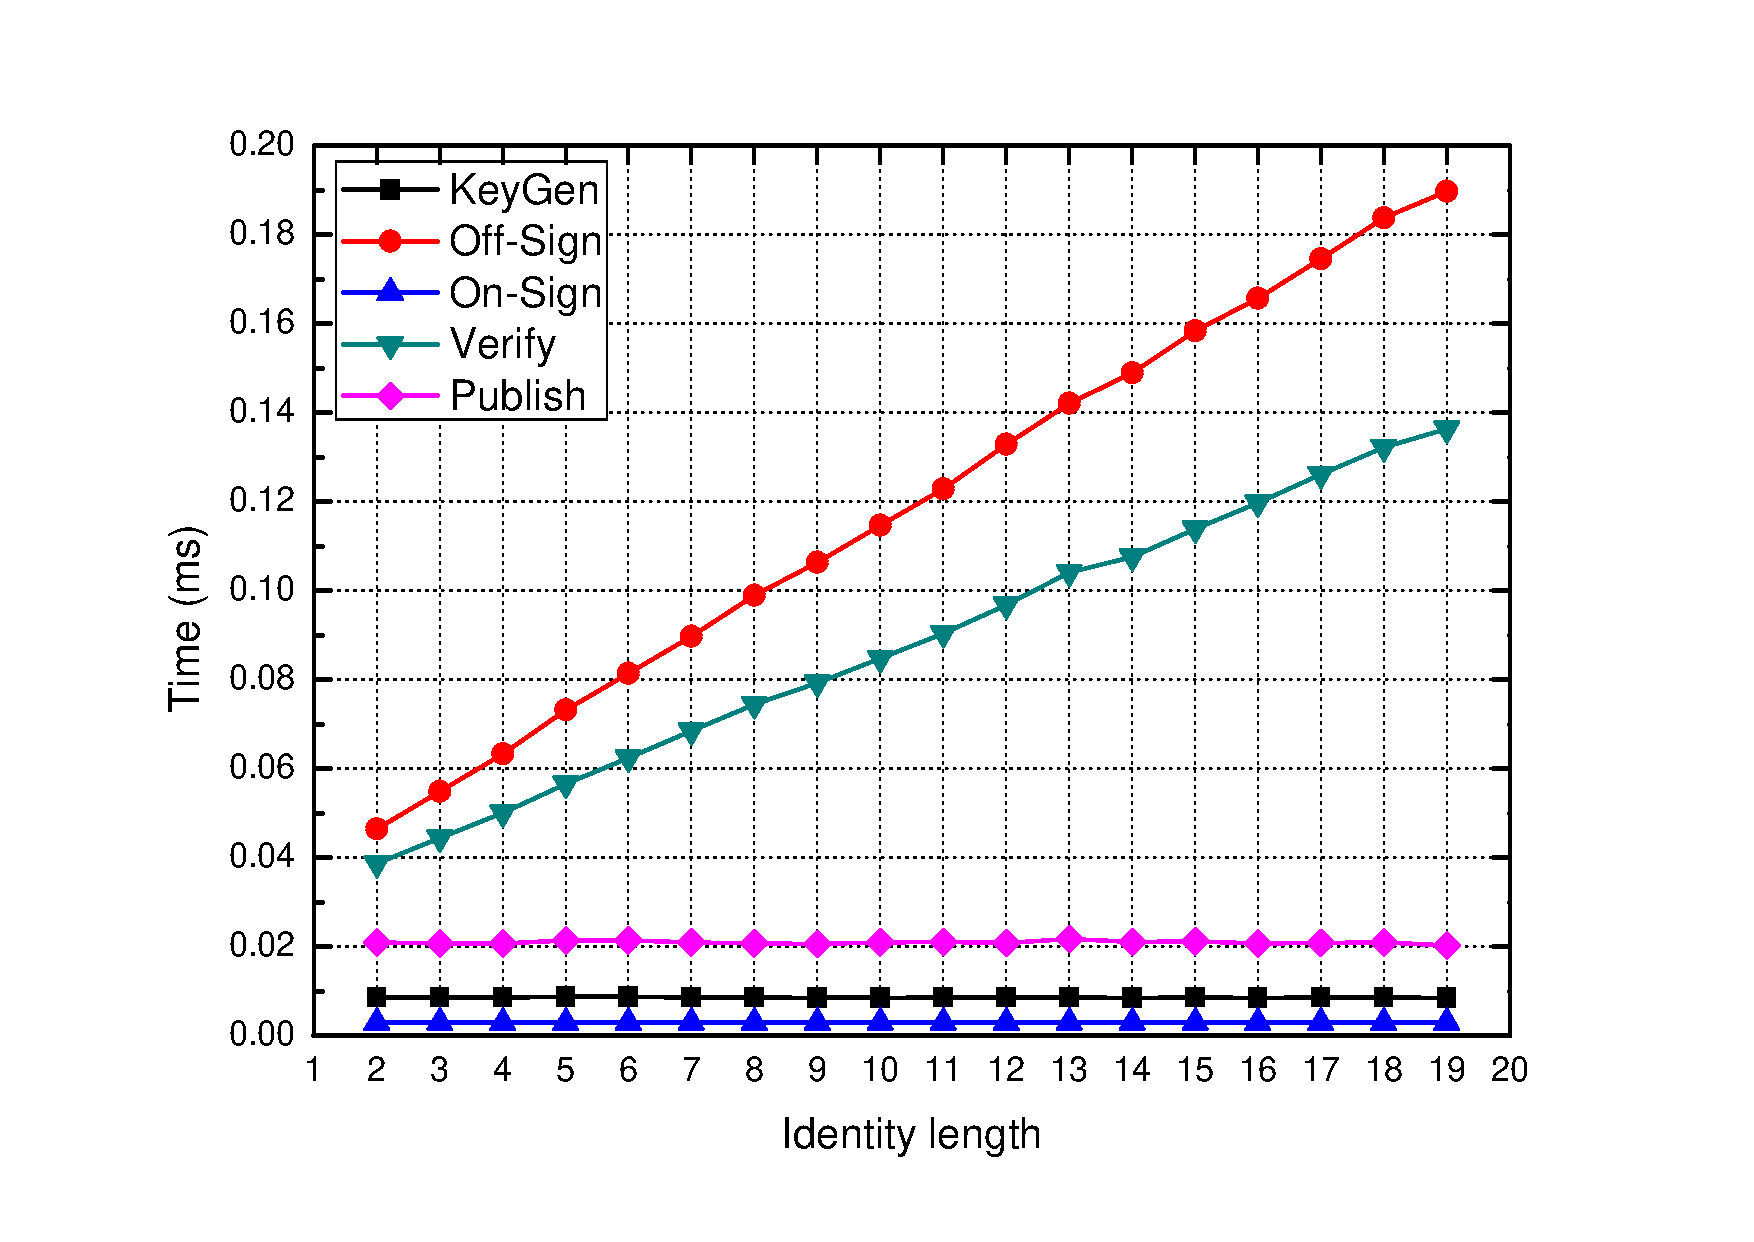
\includegraphics[width=7.5cm]{computationcost.pdf}
\caption{Algorithm computaional costs. } \label{fig-cost}
\end{figure}

The results show that the computational costs of \emph{Offline Signing} and \emph{Verification} algorithms scale linearly as the identity lengths increase, while the costs of \emph{KeyGen}, \emph{Publish} and \emph{Online Signing} algorithms are basically constants. 
Apparently, \emph{Online Signing} is mush faster than \textit{Offline Signing} algorithm.
Let $k$ be the length of an identity, evaluation shows that \emph{Online Signing} is above 15 times faster than \textit{Offline Signing} when $k = 2$, and rises to above 62 times when $k = 19$.
Because a user performs offline signing beforehand and only executes the online signing when messages are ready, our online/offline model can effectively improve the signing efficiency.

\subsection{Scheme Comparison}
We theoretically compare the performance of our HIBOOS scheme with other schemes in Table \ref{table-performance}. 
Online/offline signing algorithm computation, verifying algorithm computation are compared between the the schemes.
The $q$ denotes the order of group, $k$ denotes the length of identity, $E$ represents a group exponentiation computation and $P$ represents a pairing computation.
Since the overhead of hash computation and group point multiplicative computation are negligible comparing with the $E$ and $P$ computation, we don not take them into consideration in our scheme comparison. 
\par

\begin{table*}
\centering
\caption{\label{table-performance} Comparison of different schemes. H denotes hierarchical, OO denotes online/offline model, EF denotes escrow-free model. (* The computation overhead depends on the value a random  $\beta \in \mathbb{Z}^*_q$, which up to $\left|q\right| -1$)}
\begin{tabular}{|c|c|c|c|c|c|c|}
\hline
Scheme &H &OO &EF &Offline Sign Comp. &Online Sign Comp. &Verify Comp.\\
\hline
\hline
SHER-IBS \cite{chow2004secure} &$\surd$ &$\times$ &$\times$ &$-$ &$(k+2)E$ &$(k+1)E+(k+2)P$ \\
\hline
K-IBOOS \cite{kar2014provably} &$\times$ &$\surd$ &$\times$ &$(\left| q\right| -1)P$ &* &$1E+3P$ \\
\hline
CWS-HIBOOS\cite{chen2015ahiboos} &$\surd$ &$\surd$ &$\times$ &$(2k+2)E+2P$ &$2E$ &$(k+1)E+(k+2)P$ \\
\hline
CWS-EF-HIBS\cite{anescrowfree2015chen} &$\surd$ &$\times$ &$\surd$ &$-$ &$(k+3)E$ &$(k+1)E+(k+3)P$ \\
\hline
Our scheme &$\surd$ &$\surd$ &$\surd$ &$(2k+3)E+(k+1)P$ &$2E$ &$(k+1)E+(k+2)P$ \\
\hline
\end{tabular}
\end{table*}

Although introducing heavy computations, especially the three pairing computations in the offline singing phase, our HIBOOS scheme can achieve high online efficiency that the computation overhead is constant, which is also better than the K-IBOOS scheme.
Our HIBOOS scheme extends the CWS-HIBOOS scheme \cite{chen2015ahiboos}.
The comparing results show that our escrow-free scheme introduces low extra overhead to the primitive HIBOOS scheme.  
\par

\section{Related Work} \label{sec-relatedwork}
Even et al. first introduce the notion of online/offline signatures to reduce the computational cost of signature generation \cite{even1990line}.
An OO signature scheme divides the process of message signing into offline phase and online phase.
The offline phase with most of the heavy computations is performed prior to obtaining the message to be signed.
And the online phase performing the light computations is executed when messages are ready.
According to the OO signature model, several identity-based online/offline signature scheme have been proposed \cite{liu2011online,yasmin2010authentication,liu2010efficient,kar2014provably}.
Liu et al. propose an online/offline IBS scheme (LJY-IBOOS) for securing wireless sensor network \cite{liu2010efficient}.
Yang et al. illuminate that the LJY-IBOOS scheme is not secure and propose an identity-based online/offline threshold signature scheme, which achieves higher security \cite{yang2013id}.
Both of their schemes are not appropriate for hierarchical IBS.
Since each cryptosystem needs to be proved security utilizing formal mathematical methodology, it cannot directly extend a proved-secure IBS scheme to a secure HIBS scheme.
Moreover, a secure HIBS scheme has to solve the domain-PKG collusion problem in addition. 
\par

Works on key escrow problem can be categorized into two types: IBC-applicable solutions \cite{boneh2001identity,kate2010distributed,lee2004secure,cao2011sa,wang2015thibe} and IBS-applicable solutions \cite{zhang2012efficient,yuen2010construct,ogiela2012linguistic}.
\textbf{IBC-applicable solution}. This type of solutions can be apply to solve the key escrow problems in both the (H)IBE and (H)IBS schemes.
Most of the solutions impose extra organizations to distribute the ability of PKG so that a single PKG is not able to generate and obtain user private keys.  
Boneh et al. first apply the threshold method to suggest an multi-PKG mechanism \cite{boneh2001identity}. 
Kate and Goldberg improve their model and apply the model to three well-known IBE schemes \cite{kate2010distributed}. 
Besides, some researchers introduce Key Privacy Authorities (KPAs) to restrict the power of PKG \cite{lee2004secure,cao2011sa,wang2015thibe}. 
However, either the multi-PKG or PKG-KPAs models brings significant overhead because of the extra identity authentication and the more complicated key generating algorithms.
\textbf{IBS-applicable solution}. This type of solutions relies on the fact that the signer can attach extra information to the signature so that the message receivers can utilize the information along with the public key of the signer to verify the signature.
Yuen et al. propose an escrow-free IBS model that each signer uses a public key and a secret key to sign messages \cite{yuen2010construct}. 
Two signatures are generated and verified for one message.
Besides, a judge and a Trusted Third Party are required in their model.
Zhang et al. propose an escrow-free IBS scheme that unnecessarily depends on any judges \cite{zhang2012efficient}. 
The essence of their scheme is that a user-selected secret is added while generating the private key so that the PKG cannot obtain a complete key. 
However, either Yuen's model or Zhang's scheme is only for IBS schemes. 

\section{Conclusion}\label{sec-conclusion}
In this paper we propose a provably-secure escrow-free hierarchical Identity-based Online/Offline Signature scheme.
The main idea of the escrow-free model lay on 1) imposing user-selected secret while signing message so as to restrict the PKGs' ability of generating an identical signature as user; and 2) introducing PKG signing factor to the signature so that the user could not generate well-formed signatures with different user parameter.
According to the idea, we presented an escrow-free HIBOOS scheme based on the CWS-HIBOOS scheme.
Based on the CDH assumption, we proved the security of our escrow-free HIBOOS scheme.
Our scheme only introduced acceptable overhead to the CWS-HIBS scheme and our escrow-free model was flexible and compatible to the primitive schemes. 
\par

\ack This work was partially supported by National Science Foundation of China(NSFC) under grant no. 61303264; National Science Foundation of China(NSFC) under grant no. 61202488, and also in part supported by Soonchunhyang University Research Fund; the Basic Science Research Program through the National Research Foundation of Korea (NRF) funded by the Ministry of Science, ICT and Future Planning (2014R1A1A1005915).


\begin{thebibliography}{10}

\bibitem{campbell2008rise}
A.~T. Campbell, S.~B. Eisenman, N.~D. Lane, E.~Miluzzo, R.~Peterson, H.~Lu,
  X.~Zheng, M.~Musolesi, K.~Fodor, G.-S. Ahn \emph{et~al.}, The rise of
  people-centric sensing, \emph{Internet Computing, IEEE}, vol.~12, no.~4,
  pp. 12--21, 2008.

\bibitem{cornelius2008anonysense}
C.~Cornelius, A.~Kapadia, D.~Kotz, D.~Peebles, M.~Shin, and N.~Triandopoulos,
  Anonysense: privacy-aware people-centric sensing, \emph{Proceedings of
  the 6th international conference on Mobile systems, applications, and
  services}.\hskip 1em plus 0.5em minus 0.4em\relax ACM, 2008, pp. 211--224.

\bibitem{shi2010prisense}
J.~Shi, R.~Zhang, Y.~Liu, and Y.~Zhang, Prisense: privacy-preserving data
  aggregation in people-centric urban sensing systems, \emph{INFOCOM, 2010
  Proceedings IEEE}.\hskip 1em plus 0.5em minus 0.4em\relax IEEE, 2010, pp.
  1--9.

\bibitem{puttaswamy2010preserving}
K.~P. Puttaswamy and B.~Y. Zhao, Preserving privacy in location-based mobile
  social applications, \emph{Proceedings of the Eleventh Workshop on
  Mobile Computing Systems \& Applications}.\hskip 1em plus 0.5em minus
  0.4em\relax ACM, 2010, pp. 1--6.

\bibitem{johnson2007people}
P.~Johnson, A.~Kapadia, D.~Kotz, N.~Triandopoulos, and N.~Hanover,
  People-centric urban sensing: Security challenges for the new paradigm,
  \emph{Dept. of Computer Science, Dartmouth College. URL http://www. cs.
  dartmouth. edu/\~{} dfk/papers/johnson-metrosec-challenges-tr.
  pdf.--Zugriffsdatum}, vol.~26, 2007.

\bibitem{shamir1985identity}
A.~Shamir, Identity-based cryptosystems and signature schemes, in
  \emph{Advances in cryptology}.\hskip 1em plus 0.5em minus 0.4em\relax
  Springer, 1985, pp. 47--53.

\bibitem{choon2002identity}
J.~C. Choon and J.~H. Cheon, An identity-based signature from gap
  diffie-hellman groups, \emph{Public key cryptography—PKC 2003}.\hskip
  1em plus 0.5em minus 0.4em\relax Springer, 2002, pp. 18--30.
  
\bibitem{gentry2002hierarchical}
C.~Gentry and A.~Silverberg.
\newblock Hierarchical id-based cryptography.
\newblock In {\em Advances in cryptology—ASIACRYPT 2002}, pages 548--566.
  Springer, 2002.  

\bibitem{chow2004secure}
S.~S. Chow, L.~C. Hui, S.~M. Yiu, and K.~Chow, Secure hierarchical identity
  based signature and its application, \emph{Information and
  Communications Security}.\hskip 1em plus 0.5em minus 0.4em\relax Springer,
  2004, pp. 480--494.
  
\bibitem{boneh2001short}
D.~Boneh, B.~Lynn, and H.~Shacham.
\newblock Short signatures from the weil pairing.
\newblock In {\em Advances in Cryptology—ASIACRYPT 2001}, pages 514--532.
  Springer, 2001.

\bibitem{camenisch2004signature}
J.~Camenisch and A.~Lysyanskaya.
\newblock Signature schemes and anonymous credentials from bilinear maps.
\newblock In {\em Advances in Cryptology--CRYPTO 2004}, pages 56--72. Springer,
  2004.
  
\bibitem{boneh2004short}
D.~Boneh and X.~Boyen.
\newblock Short signatures without random oracles.
\newblock In {\em Advances in Cryptology-EUROCRYPT 2004}, pages 56--73.
  Springer, 2004.    

\bibitem{yao2014novel}
Y.~Yao, and Z.~Li, A novel fuzzy identity based signature scheme based on the short integer solution problem,
\emph{Computers \& Electrical Engineering},
vol. 40, no. 6, pp. 1930--1939, Elsevier 2014.


\bibitem{gerbush2012dual}
M.~Gerbush, A.~Lewko, A.~O’Neill, and B.~Waters, Dual form signatures: An
  approach for proving security from static assumptions, \emph{Advances in
  Cryptology--ASIACRYPT 2012}.\hskip 1em plus 0.5em minus 0.4em\relax Springer,
  2012, pp. 25--42.

\bibitem{boneh2001identity}
D.~Boneh and M.~Franklin, Identity-based encryption from the weil pairing,
  in \emph{Advances in Cryptology—CRYPTO 2001}.\hskip 1em plus 0.5em minus
  0.4em\relax Springer, 2001, pp. 213--229.
  
\bibitem{even1990line}
S.~Even, O.~Goldreich, and S.~Micali, On-line/off-line digital signatures,
  in \emph{Advances in Cryptology—CRYPTO’89 Proceedings}.\hskip 1em plus
  0.5em minus 0.4em\relax Springer, 1990, pp. 263--275.

\bibitem{liu2011online}
J.~K. Liu, J.~Baek, and J.~Zhou, Online/offline identity-based signcryption
  revisited, \emph{Information Security and Cryptology}.\hskip 1em plus
  0.5em minus 0.4em\relax Springer, 2011, pp. 36--51.

\bibitem{yasmin2010authentication}
R.~Yasmin, E.~Ritter, and G.~Wang, An authentication framework for wireless
  sensor networks using identity-based signatures, \emph{Computer and
  Information Technology (CIT), 2010 IEEE 10th International Conference
  on}.\hskip 1em plus 0.5em minus 0.4em\relax IEEE, 2010, pp. 882--889.

\bibitem{liu2010efficient}
J.~K. Liu, J.~Baek, J.~Zhou, Y.~Yang, and J.~W. Wong, Efficient
  online/offline identity-based signature for wireless sensor network,
  \emph{International Journal of Information Security}, vol.~9, no.~4, pp.
  287--296, 2010.

\bibitem{kar2014provably}
J.~Kar, Provably secure online/off-line identity-based signature scheme for
  wireless sensor network.'' \emph{IJ Network Security}, vol.~16, no.~1, pp.
  29--39, 2014.
    
\bibitem{lai2015improved}
J.~Lai, Y.~Mu, F.~Guo, and W.~Susilo. Improved Identity-Based Online/Offline Encryption, \emph{Information Security and Privacy, Springer International Publishing}, pp. 160--173, 2015.

\bibitem{yang2013id}
X.~Yang, C.~Li, T.~Xu, and C.~Wang, Id-based on-line/off-line
  threshold signature scheme without bilinear pairing, \emph{Journal on
  Communications}, vol.~8, 2013.
  
\bibitem{kate2010distributed}
A.~Kate and I.~Goldberg, Distributed private-key generators for
  identity-based cryptography, \emph{Security and Cryptography for
  Networks}.\hskip 1em plus 0.5em minus 0.4em\relax Springer, 2010, pp.
  436--453.

\bibitem{cao2011sa}
D.~Cao, X.-F. Wang, F.~Wang, Q.-L. Hu, and J.-S. Su, Sa-ibe: A secure and
  accountable identity-based encryption scheme, \emph{Dianzi Yu Xinxi
  Xuebao(Journal of Electronics and Information Technology)}, vol.~33, no.~12,
  pp. 2922--2928, 2011.
  
\bibitem{lee2004secure}
B.~Lee, C.~Boyd, E.~Dawson, K.~Kim, J.~Yang, and S.~Yoo.
\newblock Secure key issuing in id-based cryptography.
\newblock In {\em Proceedings of the second workshop on Australasian
  information security, Data Mining and Web Intelligence, and Software
  Internationalisation-Volume 32}, pages 69--74. Australian Computer Society,
  Inc., 2004.  

\bibitem{wang2015thibe}
X.~Wang, P.~Chen, H.~Zhou, and J.~Su.
\newblock T-hibe: A trustworthy and secure hierarchical identity-based
  encryption system [in press].
\newblock {\em Chinese Journal of Electronics}, page~0, 2015.

\bibitem{zhang2012efficient}
Y.~Zhang, J.~K. Liu, X.~Huang, M.~H. Au, and W.~Susilo, Efficient escrow-free
  identity-based signature, \emph{Provable Security}.\hskip 1em plus 0.5em
  minus 0.4em\relax Springer, 2012, pp. 161--174.

\bibitem{yuen2010construct}
T.~H. Yuen, W.~Susilo, and Y.~Mu, How to construct identity-based signatures
  without the key escrow problem, \emph{International Journal of Information
  Security}, vol.~9, no.~4, pp. 297--311, 2010.

\bibitem{ogiela2012linguistic}
M.~R.~Ogiela,U.~Ogiela, Linguistic protocols for secure information management and sharing,
\emph{Computers \& Mathematics with Applications},
vol.~63, no.~2, pp. 564--572, 2012. Elsevier, 2012.

\bibitem{chen2015efhibs}
P.~Chen, X.~Wang, S.~Hao, and J.~Su, An escrow-free hierarchical
  identity-based signature scheme from composite order bilinear groups [in
  press], \emph{The Fifth International Workshop on Cloud, Wireless and
  e-Commerce Security (CWECS 2015)}.\hskip 1em plus 0.5em minus 0.4em\relax
  IEEE, 2015.

\bibitem{joux2003separating}
A.~Joux and K.~Nguyen, Separating decision diffie--hellman from computational
  diffie--hellman in cryptographic groups, \emph{Journal of cryptology},
  vol.~16, no.~4, pp. 239--247, 2003.

\bibitem{Pointcheval1996security}
D.~Pointcheval and J.~Stern, Security proofs for signature schemes, in
  \emph{Advances in Cryptology—EUROCRYPT’96}.\hskip 1em plus 0.5em minus
  0.4em\relax Springer, 1996, pp. 387--398.
  
\bibitem{anescrowfree2015chen}
P.~Chen, X.~Wang, and J.~Su, An Escrow-Free Hierarchical Identity-Based Signature Model for Cloud Storage, 
\emph{Algorithms and Architectures for Parallel Processing}, Springer International Publishing, pp. 633--647, 2015.
Springer, 2015.  

\bibitem{pbclib}
B.~Lynn, The Pairing-Based Cryptography Library. Available at https://crypto.stanford.edu/pbc/

\bibitem{chen2015ahiboos}
P.~Chen, X.~Wang, and J.~Su, An Online/Offline HIBS Scheme for Privacy Protection of People-Centric Sensing [in press], 
\emph{2015 International Conference on Industrial Informatics --Computing Technology, Intelligent Technology, Industrial Information Integration (ICIICII 2015)}.
IEEE, 2015.

\end{thebibliography}

\end{document}
